\documentclass[fleqn]{article}
\oddsidemargin 0.0in
\textwidth 6.0in
\thispagestyle{empty}
\usepackage{import}
\usepackage{amsmath}
\usepackage{graphicx}
\usepackage{flexisym}
\usepackage{calligra}
\usepackage{amssymb}
\usepackage{bigints} 
\usepackage[english]{babel}
\usepackage[utf8x]{inputenc}
\usepackage{float}
\usepackage[colorinlistoftodos]{todonotes}


\DeclareMathAlphabet{\mathcalligra}{T1}{calligra}{m}{n}
\DeclareFontShape{T1}{calligra}{m}{n}{<->s*[2.2]callig15}{}
\newcommand{\scriptr}{\mathcalligra{r}\,}
\newcommand{\boldscriptr}{\pmb{\mathcalligra{r}}\,}

\definecolor{hwColor}{HTML}{442020}

\begin{document}

  \begin{titlepage}

    \newcommand{\HRule}{\rule{\linewidth}{0.5mm}}

    \center

    \begin{center}
      
\includegraphics[height=11cm, width=11cm]{asu.png}
    \end{center}

    \vline

    \textsc{\LARGE Classical Parts/Field/Matter III}\\[1.5cm]

    \HRule \\[0.5cm]
    { \huge \bfseries Homework 8}\\[0.4cm] 
    \HRule \\[1.0cm]

    \textbf{Behnam Amiri}

    \bigbreak

    \textbf{Prof: Samuel Teitelbaum}

    \bigbreak

    \textbf{{\large \today}\\[2cm]}

    \vfill

  \end{titlepage}

  \begin{enumerate}
    \item \textbf{10.15 (60 points)} A particle of charge $q$ moves in a circle of radius $a$ at constant
    angular velocity $\omega$. (Assume that the circle lies in the x y plane, centered at the
    origin, and at time $t = 0$ the charge is at $(a, 0)$, on the positive x axis.) Find the
    Liénard-Wiechert potentials for points on the $z$ axis.

        % \textcolor{hwColor}{
        %   \\
        % }

    \item \textbf{10.16 (20 points)} Show that the scalar potential of a point charge moving with constant 
    velocity (Eq. $10.49$) can be written more simply as
    $$
      V(r,t)=\dfrac{1}{4 \pi \epsilon_0} \dfrac{q}{R\sqrt{1-v^2 ~ sin^2 ~ \theta/c^2}},
    $$
    where $R \equiv r-vt$ is the vector from the present $(!)$ position of the particle to the
    field point $r$, and $\theta$ is the angle between $R$ and $v$ (Fig. 10.9). Note that 
    for nonrelativistic velocities $(v^2 << c^2)$,
    $$
      V(r,t) \approx \dfrac{1}{4 \pi \epsilon_0} \dfrac{q}{R}
    $$
    \emph{Note the denominator looks a lot like the lorentz factor.}
    \begin{center}
      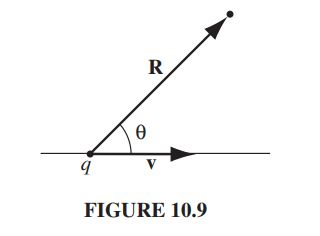
\includegraphics[height=5cm, width=7cm]{1.JPG}
    \end{center}

        % \textcolor{hwColor}{
        %   \\
        % }

    \item \textbf{10.25 (20 points)} Figure $2.35$ summarizes the laws of electrostatics in a "triangle
    diagram" relating the source $(\rho)$, the field $(E)$, and the potential $(V)$. Figure $5.48$
    does the same for magnetostatics, where the source is $J$, the field is $B$, and the
    potential is A. Construct the analogous diagram for electrodynamics, with sources
    $\rho$ and $J$ (constrained by the continuity equation), fields $E$ and $B$, and potentials $V$
    and $A$ (constrained by the Lorenz gauge condition). Do not include formulas for $V$
    and $A$ in terms of $E$ and $B$.
    \begin{center}
      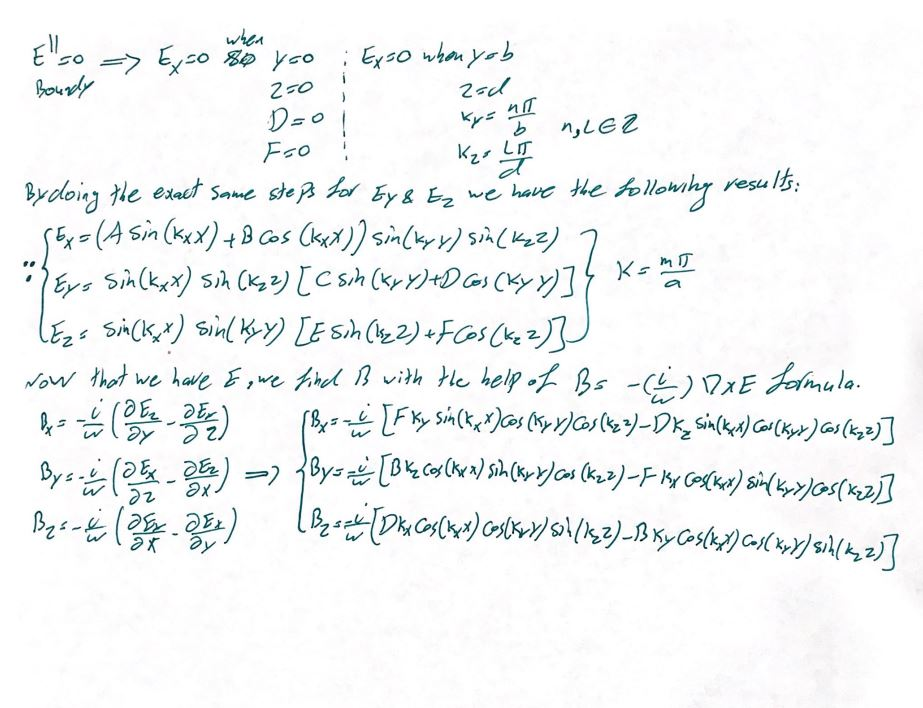
\includegraphics[height=7cm, width=7cm]{2.JPG}
    \end{center}

        % \textcolor{hwColor}{
        %   \\
        % }
    
  \end{enumerate}

\end{document}
